\textbf{PARTIE A}

\medskip

On définit sur l’intervalle $\intervOO{0}{+\infty}$ la fonction $g$ par : \[ g(x)=\frac2x - \frac{1}{x^2}+\ln(x) \text{ où } \ln \text{ désigne la fonction logarithme népérien. } \]
On admet que la fonction $g$ est dérivable sur $\intervOO{0}{+\infty} = I$ et on note $g'$ sa fonction dérivée.

\begin{enumerate}
	\item Montrer que pour $x > 0$, le signe de $g'(x)$ est celui du trinôme du second degré $\big(x^2-2x+2\big)$
	\item En déduire que la fonction g est strictement croissante sur $\intervOO{0}{+\infty}$.
	\item Montrer que l’équation $g(x) = 0$ admet une unique solution sur l’intervalle $\intervFF{0,5}{1}$, que l’on notera $\alpha$.
	\item On donne le tableau de signes de $g$ sur l’intervalle $\intervOO{0}{+\infty} = I$ :
	%
	\begin{center}
		\begin{tikzpicture}[double distance=4pt]
			\tkzTabInit{$x$/1,$g(x)$/1}{$0$,$\alpha$,$+\infty$}
			\tkzTabLine{d,-,z,+,}
		\end{tikzpicture}
	\end{center}
	%
	Justifier ce tableau de signes à l’aide des résultats obtenus aux questions précédentes.
\end{enumerate}

\medskip

\textbf{PARTIE B}

\medskip

On considère la fonction $f$ définie sur l’intervalle $\intervOO{0}{+\infty} = I$ par : \[ f(x)=\e^x \ln(x). \]
On note $\mathcal{C}_f$ la courbe représentative de $f$ dans un repère orthonormé.

\begin{enumerate}
	\item On admet que la fonction $f$ est deux fois dérivable sur $\intervOO{0}{+\infty}$, on note $f'$ sa fonction dérivée, $f''$ sa fonction dérivée seconde et on admet que, pour tout nombre réel $x > 0$ : \[ f'(x)=\e^x \left(\frac1x+\ln(x)\right). \]
	%
	Démontrer que, pour tout réel $x > 0$, on a : $f''(x) = \e^x \left(\frac2x-\frac{1}{x^2}+\ln(x)\right)$.
	
	\smallskip
	
	On pourra remarquer que pour tout réel $x > 0$, $f''(x) = \e^x \times g(x)$, où $g$ désigne la fonction étudiée dans la partie \textbf{A}.
	\item 
	\begin{enumerate}
		\item Dresser le tableau de signes de la fonction $f$ sur $\intervOO{0}{+\infty}$. Justifier.
		\item Justifier que la courbe $\mathcal{C}_f$ admet un unique point d’inflexion $A$.
		\item Étudier la convexité de la fonction $f$ sur l’intervalle $\intervOO{0}{+\infty}$. Justifier.
	\end{enumerate}
	\item 
	\begin{enumerate}
		\item Calculer les limites de $f$ aux bornes de son ensemble de définition.
		\item Montrer que $f'(\alpha) = \dfrac{\e^{\alpha}}{\alpha^2}(1-\alpha)$.
		
		On rappelle que $\alpha$ est l’unique solution de l’équation $g(x) = 0$.
		\item Démontrer que $f'(\alpha)>0$ et en déduire le signe de $f'(x)$ pour $x$ appartenant à $\intervOO{0}{+\infty}$.
		\item En déduire le tableau de variations complet de la fonction $f$ sur $\intervOO{0}{+\infty}$.
	\end{enumerate}
\end{enumerate}